\chapter{指数族表示的图模型}

指数族分布已经被各种文献广泛研究,本章将讲解能被作为指数族对待的一系列图模型。
采用指数族的观点可以阐述推断算法和凸分析理论之间的一些基本联系。
更具体地说,正如我们将看到的,图模型中各类推断问题可以通过平均参数和标准参数之间的映射来理解。

\section{指数族与最大熵原理}

导出图模型指数族表示的一个基本出发点是最大熵原理。
我们首先从简单的标量随机变量 $X$ 入手,探索一下有哪些可供后来借鉴的启示。
假设有 $n$ 个独立同分布(i.i.d.)的观测值 $X^1, \dots, X^n$,我们可以计算特定函数的经验期望值——也就是
\begin{equation}
    \hat{\mu}_{\alpha} \coloneqq \frac{1}{n}\sum_{i = 1}^n\phi_{\alpha}(X^i), \quad \forall \alpha \in \mathcal{I}
\end{equation}
其中在某个集合 $\mathcal{I}$ 中的每个 $\alpha$ 都可以索引到一个函数 $\phi_{\alpha}: \mathcal{X} \rightarrow \mathbb{R}$。
例如我们设 $\phi_1(x) = x$,$\phi_2(x) = x^2$,则式 (3.1) 对应随机变量 $X$ 的一阶和二阶矩的经验估计值。
基于这个 $|\mathcal{I}|$-维的经验估计向量 $\hat{\mu} = (\hat{\mu}_{\alpha}, \alpha \in \mathcal{I})$,我们的目标是去推断随机变量 $X$ 的全概率分布。
特别地,我们将概率分布表示为关于某个测度 $\nu$ 的绝对连续的密度 $p$。
这个基本测度 $\nu$ 可以是 $\{0, 1, \dots, r-1\}$ 的计数测度,此时 $p$ 对应一个概率质量函数,或者对于连续随机向量,基本测度 $\nu$ 可以是 $\mathbb{R}$ 上的勒贝格测度。

对于一个给定的分布 $p$,假设期望值 $\mathbb{E}[\phi_{\alpha}(X)] \coloneqq \int_{\mathcal{X}}\phi_{\alpha}(x)p(x)\nu(dx)$,$\alpha \in \mathcal{I}$。
如果满足条件
$$\mathbb{E}_p[\phi_{\alpha}(X)] = \hat{\mu}_{\alpha}, \quad \forall \alpha \in  \mathcal{I}$$
我们称分布 $p$ 和数据一致。
换句话说就是在分布 $p$ 下的期望 $\mathbb{E}_p[\phi_{\alpha}(X)]$ 与经验分布一致。
一般来说有很多分布 $p$ 与数据一致,因此需要一个原则来决定选择其中一个来作为 $X$ 最佳的全概率分布。

我们引入香农熵(Shannon Entropy)
\begin{equation}
    H(p) \coloneqq -\int_{\mathcal{X}} (\log{p(x)})p(x)\nu(dx)
\end{equation}
最大熵原理是指从与数据一致的分布中选择香农熵最大的分布 $p^*$。
严格地说,令 $\mathcal{P}$ 代表随机变量 $X$ 所有可能分布的集合,最大熵解 $p^*$ 由下面的约束优化问题给出:
\begin{equation}
    p^* \coloneqq arg\max_{p \in \mathcal{P}}H(p) \quad \text{subject to } \mathbb{E}_p[\phi_{\alpha}(X)] = \hat{\mu}_{\alpha}, \quad \forall \alpha \in \mathcal{I}
\end{equation}
对最大熵原理的一种解释是在保持数据一致性的条件下选择具有最大不确定性(由熵函数 (3.2) 度量)的分布。
如果问题 (3.3) 有解,在连续情况下可以使用变分法,在离散情况下可以直接计算,最优解 $p^*$ 具有这种形式
\begin{equation}
    p_{\theta}(x) \propto \exp{\{\sum_{\alpha \in \mathcal{I}}\theta_{\alpha}\phi_{\alpha}(x)\}}
\end{equation}
其中 $\theta \in \mathbb{R}^d$ 表示指数族形式下的一组参数。
从最大熵的角度来看,参数 $\theta$ 有一个非常具体的解释,那就是和经验量 $\hat{\mu}$ 约束相关的一组拉格朗日乘子。
下面的章节中我们将对这种联系进行更为深入的探索。

\section{指数族的基础内容}

经过上面那个例子的启发之后,我们来建立指数族的标准框架。
更准确地说,指数族是建立在基本测度 $\nu$ 之上的一些参数化的密度函数。

给定取值空间为 $\mathcal{X}^m = \otimes_{s = 1}^m\mathcal{X}_s$ 的一个随机向量 $(X_1, X_2, \dots, X_m)$,令 $\phi = (\phi_{\alpha}, \alpha \in \mathcal{I})$ 为一系列函数 $\phi_{\alpha}: \mathcal{X}^m \rightarrow \mathbb{R}$ 的集合,这些函数也就是势函数(Potential functions)或者充分统计量(Sufficient Statistics)。
$\mathcal{I}$ 是一个包含 $d = |\mathcal{I}|$ 个元素的索引集,因此 $\phi$ 也可以看作是将 $\mathcal{X}^m$ 映射到 $\mathbb{R}^d$ 的向量值函数。
对于一个给定的充分统计量向量 $\phi$,令 $\theta = (\theta_{\alpha}, \alpha \in \mathcal{I})$ 代表相关的一组量,这组量被称为标准参数(Canonical Parameters)或者指数参数。
对于每个向量 $x \in \mathcal{X}^m$,我们使用 $\langle \theta, \phi(x) \rangle$ 代表 $\mathbb{R}^d$ 空间中 $\theta$ 与 $\phi(x)$ 两个向量的欧几里得内积。

采用这些符号可以把与 $\phi$ 相关的指数族表示为以下带参密度函数形式
\begin{equation}
    p_{\theta}(x_1, x_2, \dots, x_m) = \exp{\{\langle \theta, \phi(x) \rangle - A(\theta)\}}
\end{equation}
相应的测度为 $\nu$ \footnote{对于任意的可测集 $S$,我们有 $\mathbb{P}[X \in S] = \int_Sp_{\theta}(x)\nu(dx)$。}。
其中 $A$ 被称为对数配分函数(Log Partition Function)或者累积函数(Cumulant Function),由以下积分定义
\begin{equation}
    A(\theta) = \log{\int_{\mathcal{X}^m}\exp{\langle \theta, \phi(x) \rangle}\nu(dx)}
\end{equation}
假设积分存在,整个定义保证了 $p_{\theta}$ 是归一化的($\int_{\mathcal{X}^m}p_{\theta}\nu(dx) = 1$)。
对于给定的一组势函数 $\phi$,每一个参数向量 $\theta$ 对应族内的一个特定分布 $p_{\theta}$。
我们感兴趣的标准参数 $\theta$ 属于下面这个集合
\begin{equation}
    \Omega \coloneqq \{\theta \in \mathbb{R}^d| A(\theta) < +\infty\}
\end{equation}
我们很快就会看到 $A$ 是 $\theta$ 的一个凸函数,这也表示 $\Omega$ 必须是一个凸集。
对数配分函数 $A$ 在本文中有着很重要的作用。

以下概念在接下来的内容里面很重要:

正则族(Regular Families):$\Omega$ 为开集的指数族称为正则族。
尽管确实存在 $\Omega$ 为闭集的指数族(参见 Brown 的作品),但是我们在这里主要把注意力放在正则族上。

最小性(Minimal):有一类典型的指数族,对于它们的充分统计量 $\phi = (\phi_{\alpha}, \alpha \in \mathcal{I})$,不存在非零向量 $a \in \mathbb{R}^d$ 使得线性组合
$$\langle a, \phi(x) \rangle = \sum_{\alpha \in \mathcal{I}}a_{\alpha}\phi_{\alpha}(x)$$
为一个常数(在 $\nu$ 测度下几乎处处满足)。
这个条件导致了一个所谓的最小表示(Minimal Representation),其中每个分布由唯一的参数向量 $\theta$ 决定。

过完备性(Overcomplete):有时候不使用最小表示,而是采用非最小或者过完备表示(Overcomplete Representation)会很方便,也就是存在线性组合 $\langle a, \phi(x) \rangle$ 等于一个常数。
在这种情况下,参数向量 $\theta$ 的整个仿射子集都可以代表相同的一个分布。
读者可能会怀疑过完备表示的效果。
的确,从统计的角度来看这是不可取的,因为丢失了参数向量 $\theta$ 的可识别性。
然而这种过完备的概念在理解和积算法及其变体的时候将会很有帮助(参见第四章)。

表 \ref{tab:3-1} 提供了一些常见的标量指数族的例子。
注意这些族都是正则族($\Omega$ 是开集)和最小族(充分统计量 $\phi$ 线性无关)。

\begin{sidewaystable}[htbp]
\caption{
    几类常见的标量随机变量的指数族
}\label{tab:3-1}
\centering
\begin{threeparttable}
\begin{tabular}{lccccc}
    \hline
    Family & $\mathcal{X}$ & \tabincell{c}{$\nu$ \\ $h(\cdot)$} & $\langle \theta, \phi(x) \rangle$ & $A(\theta)$ & $\Omega$ \\
    \hline
    Bernoulli & $\{0, 1\}$ & Counting & $\theta x$ & $\log{[1+\exp{(\theta)}]}$ & $\mathbb{R}$ \\
    Gaussian & $\mathbb{R}$ & Lebesgue & $\theta x$ & $\frac{1}{2}\theta^2$ & $\mathbb{R}$ \\
    Location family & & $h(x) = \frac{\exp{(-x^2/2)}}{\sqrt{2\pi}}$ & & & \\
    Gaussian & $\mathbb{R}$ & Lebesgue & $\theta_1x + \theta_2x^2$ & $-\frac{\theta_1^2}{4\theta_2^2} - \frac{1}{2}\log{(-2\theta_2)}$ & $\{(\theta_1, \theta_2) \in \mathbb{R}^2| \theta_2 < 0\}$ \\
    Location-scale & & $h(x) = \frac{1}{\sqrt{2\pi}}$ & & & \\
    Exponential & $(0, +\infty)$ & Lebesgue & $\theta x$ & $-\log{(-\theta)}$ & $(-\infty, 0)$ \\
    Poison & $\{0, 1, 2, \dots\}$ & \tabincell{c}{Counting \\ $h(x) = 1/x!$} & $\theta x$ & $\exp{(\theta)}$ & $\mathbb{R}$ \\
    Beta & $(0, 1)$ & Lebesgue & \tabincell{c}{$\theta_1\log{x}$ \\ $+\theta_2\log{(1-x)}$} & \tabincell{c}{$\sum_{i = 1}^2\log{\Gamma(\theta_i+1)}$ \\ $-\log{\Gamma(\sum_{i = 1}^2(\theta_i+1))}$} & \\
    \hline
\end{tabular}
\begin{tablenotes}
    \item 注意:以上示例的基本测度 $\nu$ 要么是计数测度要么是勒贝格测度,与空间 $\mathcal{X}$ 严格相符,在某些例子中由因子 $h(\cdot)$ 进行调整。
        所有示例均为最小族和正则族。
\end{tablenotes}
\end{threeparttable}
\end{sidewaystable}

\section{指数形式的图模型示例}

表 \ref{tab:3-1} 中的标量示例可以作为更复杂的具有图结构的指数族的构建模块使用。
前面我们使用函数的乘积来描述图模型,如式 (2.1) 与 (2.2),这些乘积在指数族的形式里变成了求和。
在这里我们讨论一些常见的指数族形式的图模型示例。
熟悉这些例子的读者可以直接跳到 3.4 小节,在那里我们将继续对指数族进行一般性的讨论。

\begin{tcolorbox}
\begin{exam}[伊辛模型]

伊辛模型(Ising Model)来自于统计物理,是一个典型的指数族形式图模型。
考虑图 $G = (V, E)$,假设与节点 $s \in V$ 相关的随机变量 $X_s$ 是 Bernoulli 的,例如取“自旋”值 $\{-1, +1\}$。
在统计物理学的背景下,这些值可能代表磁场中磁极的方向,或者气体中粒子的存在或不存在。
伊辛模型及其变体也被用于图像处理和空间统计,其中 $X_s$ 可能对应于黑白图像的像素值,还可以被用于社交网络建模,例如政客的投票模式。

仅当图上节点 $s$ 和 $t$ 被边相连的时候,随机向量 $X$ 的组分 $X_s$ 和 $X_t$ 才会有直接交互。
这种设定可以导出如下密度的指数族
\begin{equation}
    p_{\theta}(x) = \exp{\{\sum_{s \in V}\theta_sx_s + \sum_{(s, t) \in E}\theta_{st}x_sx_t - A(\theta)\}}
\end{equation}
其中基本测度 $\nu$ 为被限定在 $\{0, 1\}^m$ 上的计数测度\footnote{更准确地说,对于每个单元素集合 $\{x\}$,如果 $x \in \{0, 1\}^m$,则 $\nu(\{x\}) = 1$,否则 $\nu(\{x\}) = 0$,而且可以由次可加性(Sub-additivity)扩展到任意集合。}。
这里 $\theta_{st} \in \mathbb{R}$ 代表边的强度,$\theta_s \in \mathbb{R}$ 代表节点 $s$ 的势,在统计物理中模拟一个“外场”,或者在空间统计中模拟一个有噪声的观测值。
严格地说,式 (3.8) 定义的密度族比经典的伊辛模型更为一般,经典伊辛模型的 $\theta_{st}$ 对所有边都相等。

作为一个指数族,伊辛模型的索引集 $\mathcal{I}$ 为 $V \cup E$,族的维度为 $d = m + |E|$。
对数配分函数由下面的求和给出
\begin{equation}
    A(\theta) = \log{\sum_{x \in \{0, 1\}^m}\exp{\{\sum_{s \in V}\theta_sx_s + \sum_{(s, t) \in E}\theta_{st}x_sx_t\}}}
\end{equation}
由于这个求和对于所有的 $\theta \in \mathbb{R}^d$ 都是有限的,因此 $\Omega$ 为整个空间 $\mathbb{R}^d$,为正则族。
此外这是一种最小表示,因为对于势函数来说不存在结果为常数的线性组合。

标准的伊辛模型可以从许多不同的方面进行推广。
尽管式 (3.8) 只包含两两相互作用,但随机变量之间的高阶交互作用也可以包括进来。
例如,为了包含 3-团 $\{s, t, u\}$ 的耦合作用,我们可以在式 (3.8) 中再添加一项 $x_sx_tx_u$,相关的标准参数设为 $\theta_{stu}$。
更一般地,对于 $k$-团之间的耦合,我们可以添加一直到 $k$ 阶的项,统计物理学中的 $k$-自旋模型就是这么来的。
当阶数取到最高 $k = m$ 时,图模型可以表示二元随机向量 $X \in \{0, 1\}^m$ 的任意分布。

\end{exam}
\end{tcolorbox}

\begin{tcolorbox}
\begin{exam}[度量标记和波茨模型]

我们考虑伊辛模型的另一种一般化版本:假设每个节点 $s \in V$ 对应的随机变量 $X_s$ 从离散空间 $\mathcal{X} \coloneqq \{0, 1, \dots, r-1\}$ 中取值($r > 2$)。
状态 $j \in  \mathcal{X}$ 可以看作一个标签,例如图像分割问题中定义的隶属类别。
每一对节点 $s \in V$ 和状态 $j \in \mathcal{X}$ 都可以派生出一个充分统计量
\begin{equation}
    \mathbb{I}_{s;j}(x_s) = \begin{cases}
        1 & \text{如果} x_s = j \\
        0 & \text{其他}
    \end{cases}
\end{equation}
相关的标准参数向量为 $\theta_s = \{\theta_{s;j}, j = 0, \dots, r-1\}$。
此外,每条边 $(s, t)$ 和每对状态值 $(j, k) \in \mathcal{X} \times \mathcal{X}$ 也可以定义一个充分统计量
\begin{equation}
    \mathbb{I}_{st;jk}(x_s, x_t) = \begin{cases}
        1 & \text{如果} x_s = j \text{且} x_t = k \\
        0 & \text{其他}
    \end{cases}
\end{equation}
相关的标准参数为 $\theta_{st;jk} \in \mathbb{R}$。
以上定义的充分统计量可以构成一个维数为 $d = r|V| + r^2|E|$ 的指数族。
与伊辛模型相似,对数配分函数处处有限,因此这个指数族是正则的。
然而与伊辛模型不同的是,这个指数族是过完备的:充分统计量之间有很多种线性相关关系存在,例如对于任意节点 $x_s \in V$ 都有 $\sum_{j \in \mathcal{X}}\mathbb{I}_{s;j}(x_s) = 1$。

度量标记问题(Metric Labeling)是这个模型的一个特例,它引入了一个度量 $\rho: \mathcal{X} \times \mathcal{X} \rightarrow [0, \infty)$ 来确定参数,即对所有 $(j, k) \in \mathcal{X} \times \mathcal{X}$,都有 $\theta_{st;jk} = -\rho(j, k)$。
因此标准参数满足 $\forall k \in \mathcal{X}: \theta_{st;kk} = 0$,$\forall j \neq k: \theta_{st;jk} < 0$,以及逆三角不等式($\forall (j, k, l): \theta_{st;jl} \geq \theta_{st;jk} + \theta_{st;kl}$)。
这个模型的另一个特例是来自统计物理的波茨模型(Potts Model),波茨模型中对于任意的 $k \in \mathcal{X}$ 都有 $\theta_{st;kk} = \alpha$,对于任意的 $j \neq k$ 都有 $\theta_{st;jk} = \beta$。

\end{exam}
\end{tcolorbox}

接下来我们讨论一类非常重要的在连续随机变量上构建的图模型:

\begin{tcolorbox}
\begin{exam}[高斯 MRF]

给定一个无向图 $G$ 和节点集 $V = \{1, \dots, m\}$,高斯马尔可夫随机场由满足 $G$ 上马尔可夫性(参见 2.2 小节)的多元高斯随机向量 $(X_1, \dots, X_m)$ 构成。
它可以用充分统计量 $(x_s, x_s^2, s \in V; x_sx_t, (s, t) \in E)$ 表示为指数族形式。
我们定义一个 $m$ 维向量 $\theta$ 作为充分统计量 $x = (x_1, \dots, x_m)$ 的相关参数,定义一个对称矩阵 $\Theta \in \mathbb{R}^{m \times m}$ 作为矩阵 $xx^T$ 的相关参数。
根据 Hammersley-Clifford 定理,矩阵 $\Theta$ 为逆协方差阵或精度矩阵的负值,它的特点是如果 $(s, t) \notin E$,则 $\Theta_{st} = 0$,如图 \ref{fig:3-1} 所示。
最终所得的指数族的维数为 $d = 2m + |E|$。

在这种设定下,多元高斯可以表达为如下指数族形式:
\begin{equation}
    p_{\theta}(x) = \exp{\{\langle \theta, x \rangle + \frac{1}{2}\langle \langle \Theta, xx^T \rangle \rangle - A(\theta, \Theta)\}}
\end{equation}
其中 $\langle \theta, x \rangle \coloneqq \sum_{i = 1}^m\theta_ix_i$ 为 $\mathbb{R}^m$ 上的欧几里得内积,此外
\begin{equation}
    \langle \langle \Theta, xx^T \rangle \rangle \coloneqq \text{trace}(\Theta xx^T) = \sum_{i = 1}^m\sum_{j = 1}^m\Theta_{ij}x_ix_j
\end{equation}
为对称阵上的 Frobenius 内积。
仅当 $\Theta \prec 0$ 的时候积分定义的 $A(\theta, \Theta)$ 才是有限的,因此
\begin{equation}
    \Omega = \{(\theta, \Theta) \in \mathbb{R}^m \times \mathbb{R}^{m \times m}| \Theta \prec 0, \Theta = \Theta^T\}
\end{equation}

\end{exam}
\end{tcolorbox}

\begin{figure}[htbp]
    \centering
    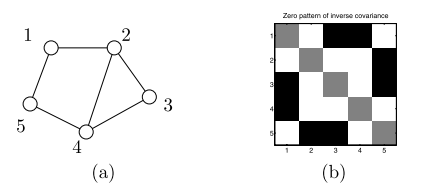
\includegraphics[width=.8\linewidth]{3-1.PNG}
    \caption{
        (a) 5 个节点的无向图模型。
        (b) 对于一个高斯马尔可夫随机场来说,它的逆协方差阵或者精度矩阵的零模式反映了图结构:对于任何一对 $i \neq j$,如果 $(i, j) \notin E$,那么 $\Theta_{ij} = 0$。
    }\label{fig:3-1}
\end{figure}

图模型并不局限于每个节点上的随机变量都属于同一指数族的情况。
更一般地,我们可以考虑指数族成员的异质组合,如下面的例子所示。

\begin{tcolorbox}
\begin{exam}[混合模型]

如图 \ref{fig:3-2}(a) 所示,一个标量混合模型的图表示十分简单。
具体说来,在一个有限混合高斯模型中,令 $X_s$ 代表一个多元变量,取值为 $\{0, 1, \dots, r-1\}$。
$X_s$ 所起的作用是对混合成分进行选择,因此我们一共有 $r$ 个成分。
和例 3.2 中描述的波茨模型一样,这个随机变量的分布是以 $\{\mathbb{I}_j[x_s], j = 0, \dots, r-1\}$ 为充分统计量,以 $\{\alpha_{s;0}, \dots, \alpha_{s;r-1}\}$ 为标准参数的指数族。

在混合模型中,给定 $X_s = j$,令 $Y_s$ 代表均值和方差为 $(\mu_j, \sigma_j^2)$ 的条件高斯。
每一个这样的条件分布都可以被写成是充分统计量为 $\{y_s, y_s^2\}$,标准参数为 $(\gamma_{s;j}, \gamma_{s;j}') \coloneqq (\frac{\mu_j}{\sigma_j^2}, -\frac{1}{2\sigma_j^2})$ 的指数族形式。
总之,我们可以得到整个模型的指数族形式,它的标准参数为
$$\theta_s \coloneqq (\underbrace{\alpha_{s;0}, \dots, \alpha_{s;r-1}}_{\alpha_s}, \underbrace{\gamma_{s;0}, \dots, \gamma_{s;r-1}}_{\gamma_s}, \underbrace{\gamma_{s;0}', \dots, \gamma_{s;r-1}'}_{\gamma_s'})$$
它的密度函数为
\begin{align}
    p_{\theta_s}(y_s, x_s) &= p_{\alpha}(x_s)p_{\gamma_s}(y_s|x_s)  \nonumber \\
    &\propto \exp{\{\sum_{j = 0}^{r-1}\alpha_{s;j}\mathbb{I}_j(x_s) + \sum_{j = 0}^{r-1}\mathbb{I}_j(x_s)[\gamma_{s;j}y_s + \gamma_{s;j}'y_s^2]\}}
\end{align}

$(X_s, Y_s)$ 为描述多元数据 $((X_1, Y_1), (X_2, Y_2), \dots, (X_m, Y_m))$ 的基本模块,可以用它来构建更加复杂的模型。
例如可以假设多元向量 $X = (X_1, \dots, X_m)$ 可以在某个基本图 $G = (V, E)$ 上构成马尔可夫随机场(参见例 3.2 中的波茨模型),变量 $Y_s$ 在给定 $\{X = x\}$ 的情况下条件独立。
根据这些可以导出一个参数为 $\theta = (\alpha, \gamma)$ 的指数族 $p_{\theta}(y, x)$,其密度为
\begin{equation}
    p_{\alpha}(x)p_{\gamma}(y|x) \propto \exp{\{\sum_{s \in V}\alpha_s(x_s) + \sum_{(s, t) \in E}\alpha_{st}(x_s, x_t)\}\prod_{s \in V}p_{\gamma_s}(y_s|x_s)}
\end{equation}
其中 $p_{\alpha}(x)$ 为波茨型(Potts-type)分布,$p_{\gamma}(y|x)$ 为局部条件分布。
$\alpha_s(x_s)$ 为 $\sum_{j = 0}^{r-1}\alpha_{s;j}\mathbb{I}_j(x_s)$ 的简写,$\alpha_{st}(x_s, x_t)$ 与此类似;非简写形式参见例 3.2。

\end{exam}
\end{tcolorbox}

\begin{figure}[htbp]
    \centering
    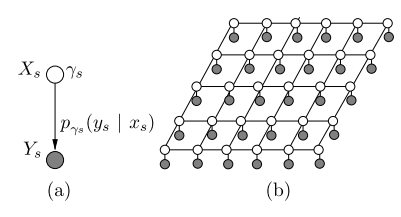
\includegraphics[width=.8\linewidth]{3-2.PNG}
    \caption{
        (a) 有限混合高斯模型的图表示:$X_s$ 为混合成分的多元标签,$Y_s$ 在给定 $X_s = j$ 的条件下是一个条件高斯量,$p_{\gamma_s}(y_s|x_s)$ 是以指数形式表示的高斯密度。
        (b) 耦合混合高斯图模型,向量 $X = (X_1, \dots, X_m)$ 是一个无向图上的马尔可夫随机场,$(Y_1, \dots, Y_m)$ 中的元素在给定 $X$ 时是条件独立的。
    }\label{fig:3-2}
\end{figure}

以上描述的混合模型存在两个层级,下面的例子存在三个层级:

\begin{tcolorbox}
\begin{exam}[隐迪利克雷分配]

隐迪利克雷分配(Latent Dirichlet Allocation,LDA)是一个典型的层次贝叶斯模型,用来捕获文档语料中词之间的统计依赖性。
模型涉及三种不同类型的随机变量:“文档(Documents)” $U$、“主题(Topics)” $Z$、“单词(Words)” $W$。
单词是分布在某个词汇表上的多元随机变量。
主题也是多元随机变量。
主题变量的每个值都与单词上的一个分布相关。
每篇文档可以看作是主题上的一个分布。
最终整个语料可以看作是文档上的一个分布。
在 LDA 模型中,语料对应的分布为迪利克雷分布。

更正式地说,单词 $W$ 取自一个多项分布,$\mathbb{P}(W = j|Z = i; \gamma) = \exp(\gamma_{ij}), \quad j = 0, 1, \dots, k-1$,其中 $\gamma_{ij}$ 代表第 $i$ 个主题下第 $j$ 个词出现的概率。
这个条件分布可以采用指示函数表达为指数族的形式:
\begin{equation}
    p_{\gamma}(w|z) \propto \exp(\sum_{i = 0}^{r-1}\sum_{j = 0}^{k-1}\gamma_{ij}\mathbb{I}_i(z)\mathbb{I}_j(w))
\end{equation}
其中 $\mathbb{I}_i(z)$ 为事件 $\{Z = i\}$ 的 $\{0, 1\}$ 指示值,$\mathbb{I}_j(w)$ 于此类似。
在层次结构的下一层(见图 \ref{fig:3-3}),主题变量 $Z$ 也遵循多项分布,其参数由迪利克雷变量确定如下:
\begin{equation}
    p(z|u) \propto \exp\{\sum_{i = 0}^{r-1}\mathbb{I}_i[z]\log u_i\}
\end{equation}
最后在层次结构的顶层,迪利克雷变量 $U$ 具有勒贝格测度下的密度形式 $p_{\alpha}(u) \propto \exp\{\sum_{i = 0}^{r-1}\alpha_i\log u_i\}$。
综上,对于一个三元组 $X \coloneqq (U, Z, W)$ 来说,LDA 模型是一个参数为 $\theta \coloneqq (\alpha, \gamma)$ 的指数族,其密度如下:
\begin{align}
    p_{\alpha}(u)p(z|u)p_{\gamma}(w|z) &\propto \exp\{\sum_{i = 0}^{r-1}\alpha_i\log u_i + \sum_{i = 0}^{r-1}\mathbb{I}_i[z]\log u_i\} \nonumber \\
    &\times \exp\{\sum_{i = 0}^{r-1}\sum_{j = 0}^{k-1}\gamma_{ij}\mathbb{I}_i[z]\mathbb{I}_j[w]\}
\end{align}

充分统计量 $\phi$ 由函数 $\{\log u_i\}$,$\{\mathbb{I}_i[z]\log u_i\}$ 和 $\{\mathbb{I}_i[z]\mathbb{I}_j[w]\}$ 构成。
如图 \ref{fig:3-3} 所示,整个 LDA 模型需要对这些局部结构进行很多次的重复。

\end{exam}
\end{tcolorbox}

\begin{figure}[htbp]
    \centering
    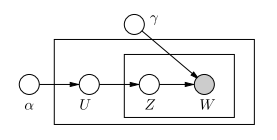
\includegraphics[width=.5\linewidth]{3-3.PNG}
    \caption{
        LDA 模型的图表示。
        单词变量 $W$ 为潜在主题 $Z$ 下的条件多元变量,其中 $\gamma$ 指定相应的分布。
        主题 $Z$ 也被建模为多元变量,分布以概率向量 $U$ 为参数,$U$ 服从参数为 $\alpha$ 的迪利克雷分布。
        该模型为层次贝叶斯模型的一个例子。
        这些矩形,也被称为盘(Plates),代表内部结构的重复。
    }\label{fig:3-3}
\end{figure}

很多图模型带有所谓的“硬核(Hard-core)”约束,这表示某些配置子集被禁止了。
这类问题的实例包括二元线性码的解码,以及其他组合优化问题(例如图匹配问题、覆盖问题、包装问题等)。
乍一看上去这样的分布族似乎不能使用指数族来表示,因为指数族中的密度 $p_{\theta}$ 都是严格正的——对于所有 $x \in \mathcal{X}^m$,都有 $p_{\theta}(x) > 0$。
在下面的例子中,我们将发现通过使用适当的基本测度 $\nu$ 可以将这些硬核约束融入到指数族框架中。

\begin{tcolorbox}
\begin{exam}[带有硬约束的模型]

产生硬核约束的一个重要领域是通信理论,特别是控错编码问题。
为了引出编码问题,假设有两个人——按照一个古老的惯例,称他们为爱丽丝和鲍勃——希望进行交流。
假设他们可以通过发送一串 01 序列进行通信,为了让问题变得具有研究意义,我们再假设连接双方的通信信道是随机的。
具体地说,在“位翻转(Bit-flipping)”信道中由爱丽丝发送的任何二进制数字都只有 $1-\epsilon$ 的概率被鲍勃正确接收。
该信道是一个概率模型,可以用条件分布来建模
$$p(y|x) \coloneqq \begin{cases}
    1 - \epsilon &\text{如果} x = y \\
    \epsilon &\text{如果} x \neq y
\end{cases}$$
其中 $x \in \{0, 1\}$ 代表爱丽丝发送的比特,$y \in \{0, 1\}$ 代表鲍勃接收的比特。

为了减少信道中的“噪声(Noisiness)”,爱丽丝和鲍勃约定以下的块编码(Block Coding)方案:不进行单个比特的传输,而是采用字节串 $(x_1, x_2, \dots, x_m)$ 进行通信,此外他们还约定只采用长度为 $m$ 总量为 $2^m$ 的字节串的一个子集。
这些特殊的字节串被称为编码字(Codewords),可以使用特定类型的图模型来定义。
具体来说,假设爱丽丝决定从满足一组校验的字节串 $x \in \{0, 1\}^m$ 中进行选择,校验形式假设为 $x_1 \oplus x_2 \oplus x_3 = 0$,其中 $\oplus$ 表示模 2 运算的加法。
考虑如下的奇偶检验集合 $F$,每一个 $a \in F$ 对一些比特子集 $N(a) \subset \{1, \dots, m\}$ 施加一个奇偶校验约束。
如果我们定义指示函数
\begin{equation}
    \psi_a(x_{N(a)}) \coloneqq \begin{cases}
        1 &\text{如果} \bigoplus_{i \in N(a)}x_i = 0 \\
        0 &\text{其他}
    \end{cases}
\end{equation}
那么二元线性码(Binary Linear Code)由满足 $\prod_{a \in F}\psi_a(x_{N(a)}) = 1$ 的所有字节串 $(x_1, x_2, \dots, x_m) \in \{0, 1\}^m$ 组成。
这些约束就是所谓的硬核约束,因为它们使得某些 $x$ 的取值概率为 0,也就把这些配置从分布的支撑集中清除了。
令 $(y_1, y_2, \dots, y_m) \in \{0, 1\}^m$ 表示鲍勃接收到的字节串,他的目的是利用这些观测结果来推断爱丽丝发送的是哪个编码字。
根据所使用的误差度量,这个解码问题对应于计算边际或者后验分布的众数
\begin{equation}
    p(x_1, \dots, x_m|y_1, \dots, y_m) \propto \prod_{i = 1}^mp(y_i|x_i)\prod_{a \in F}\psi_a(x_{N(a)})
\end{equation}
这种分布可以用因子图来表示,比特 $x_i$ 表示为非阴影圆形变量节点,观测值 $y_i$ 表示为阴影圆形变量节点,奇偶校验指示函数表示为方块因子节点(参见图 \ref{fig:2-9})。

这个图上的编码也可以被看作是一个指数族,只要我们对合适的基础测度取密度。
具体地说,我们可以使用奇偶校验来定义限制在有效编码字上的计数测度
\begin{equation}
    \nu(\{x\}) \coloneqq \prod_{a \in F}\psi_a(x_{N(a)})
\end{equation}
此外,由于观测值 $y_i$ 是固定的,因此条件分布 $p(y_i|x_i)$ 可以看作是 $x_i$ 的函数 $q(\cdot)$。
不用多少计算可以把这个函数写成如下指数形式
\begin{equation}
    q(x_i; \theta_i) = \exp\{\theta_ix_i - \log(1+\exp(\theta_i))\}
\end{equation}
其中指数参数 $\theta_i$ 由观测值 $y_i$ 与条件分布 $p(y_i|x_i)$ 定义为 $\theta_i = \log p(y_i|1)/p(y_i|0)$。
在二元对称信道的特殊情况下,这些标准参数可以写成
\begin{equation}
    \theta_i = (2y_i - 1)\log \frac{1-\epsilon}{\epsilon}
\end{equation}
需要注意的是我们将观测值向量 $(y_1, y_2, \dots, y_m)$ 看作是固定的。
在这样的条件下分布 (3.21) 可以作为一个指数族,其中密度是在限制计数测度 (3.22) 上定义的,形式为 $p_{\theta}(x|y) \propto \exp\{\sum_{i = 1}^m\theta_ix_i\}$。

\end{exam}
\end{tcolorbox}

\section{均值参数化和推断问题}

到目前为止,我们已经用标准参数向量 $\theta \in \Omega$ 刻画了任意指数族 $p_{\theta}$。
我们将在本节讨论任意指数族的均值参数(Mean Parameters)向量的替代参数化。
很多的统计计算,包括边缘化和最大似然估计,都可以理解为从一种参数表示到另一种参数表示的变换。

我们暂时离开主题,对边缘化问题中的观测变量或条件作用做一个评论。
如前所述,图模型的应用常常涉及到对随机变量(例如观测变量 $Y$)子集的约束,然后需要计算在后验分布 $p_{\theta}(x|y)$ 的边际。
例 3.6 中讨论的编码纠错就是这样的一个例子。
为了在接下来的讨论中简化表示,我们不再直接引用观测变量,而是只考虑指数族的无条件形式来讨论边缘化和其他计算问题。
这么做并不会损失一般性,因为观测变量的影响总可以通过适当地修正标准参数 $\theta$ 或充分统计量 $\phi$ 来解决。
(例如在例 3.6 中节点 $i$ 的噪声观测值 $y_i$ 为指数族分解提供了一个新的因子 $\exp(\theta_ix_i)$,如式 (3.23) 所示。)

\subsection{均值参数空间和边际多面体}

设 $p$ 为基本测度 $\nu$ 下的密度函数,我们暂时不假定 $p$ 为测度 $\nu$ 下的指数族。
与充分统计量 $\phi_{\alpha}: \mathcal{X}^m \rightarrow \mathbb{R}$ 相关的均值参数 $\mu_{\alpha}$ 定义为如下期望
\begin{equation}
    \mu_{\alpha} = \mathbb{E}_p[\phi_{\alpha}(X)] = \int \phi_{\alpha}(x)p(x)\nu(dx), \quad \forall \alpha \in \mathcal{I}
\end{equation}
通过这种方式,我们可以定义任意分布 $p$ 的均值参数向量 $(\mu_1, \dots, \mu_d)$,其中每个成分对应于一个充分统计量 $\phi_{\alpha}$($|\mathcal{I}| = d$)。
我们感兴趣的一个内容是向量 $u \in \mathbb{R}^d$ 随 $p$ 的改变而生成的轨迹空间。
正式而言,我们定义集合
\begin{equation}
    \mathcal{M} \coloneqq \{\mu \in \mathbb{R}^d| ~\exists ~p ~\text{s.t.} ~\mathbb{E}_p[\phi_{\alpha}(X)] = \mu_{\alpha}, ~\forall \alpha \in \mathcal{I}\}
\end{equation}
该集合包含了所有可能的均值参数。
值得注意的是,在这个定义中我们没有将密度 $p$ 限制为与充分统计量 $\phi$ 和基础测度 $\nu$ 相关的指数族。
然而在适当的条件下这个向量可以为指数族提供另一种参数化方法。

我们沿用前面一个例子来对这些概念进行说明:

\begin{tcolorbox}
\begin{exam}[高斯 MRF 的均值参数]

利用例 3.3 中高斯马尔可夫随机场的正则参数化(标准参数化),其充分统计量代表了均值参数,因此高斯马尔可夫随机场的均值参数为二阶矩矩阵 $\Sigma \coloneqq \mathbb{E}[XX^T] \in \mathbb{R}^{m \times m}$ 和均值向量 $\mu = \mathbb{E}[X] \in \mathbb{R}^m$。
对于这个特定的模型,可以直接给出所有可能的均值参数 $(\mu, \Sigma)$ 构成的集合 $\mathcal{M}$。
首先,如果 $(\mu, \Sigma)$ 是由某种分布(不一定非得是高斯)给出的,那么 $\Sigma - \mu\mu^T$ 一定是随机向量 $X$ 的一个有效协方差阵,这意味着半正定条件(Positive Semidefiniteness Condition,PSD)$\Sigma - \mu\mu^T \succeq 0$ 一定成立。
反之,对于任意满足 PSD 约束的 $(\mu, \Sigma)$,我们可以构造一个均值为 $\mu$,协方差(可能退化)为 $\Sigma - \mu\mu^T$ 的多元高斯分布,再从中导出 $(\mu, \Sigma)$。
到此为止,我们已经为高斯马尔可夫随机场建立了均值参数空间,$\mathcal{M}$ 的形式为
\begin{equation}
    \mathcal{M} = \{(\mu, \Sigma) \in \mathbb{R}^m \times \mathcal{S}_+^m| \Sigma - \mu\mu^T \succeq 0\}
\end{equation}
其中 $\mathcal{S}_+^m$ 代表 $m \times m$ 对称半正定矩阵集合。
图 \ref{fig:3-4} 给出了这个集合的标量实例($m = 1$),其中均值参数 $\mu = \mathbb{E}[X]$ 和 $\Sigma_{11} = \mathbb{E}[X^2]$ 必须满足二次约束 $\Sigma_{11} - \mu^2 \geq 0$。

\end{exam}
\end{tcolorbox}

\begin{figure}[htbp]
    \centering
    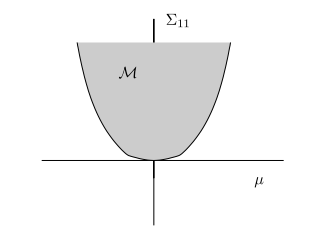
\includegraphics[width=.5\linewidth]{3-4.PNG}
    \caption{
        标量高斯的 $\mathcal{M}$ 集:这个模型具有两个均值参数 $\mu = \mathbb{E}[X]$ 和 $\Sigma_{11} = \mathbb{E}[X^2]$,必须满足二次约束 $\Sigma_{11} - \mu^2 \geq 0$。
        注意 $\mathcal{M}$ 是凸集,这个性质具有普遍性。
    }\label{fig:3-4}
\end{figure}

集合 $\mathcal{M}$ 总是 $\mathbb{R}^d$ 的一个凸子集。
可以证明,如果 $\mu$ 和 $\mu'$ 都是 $\mathcal{M}$ 中的元素,那么一定存在分布 $p$ 和 $p'$ 使得 $\mu = \mathbb{E}_p[\phi(X)]$ 且 $\mu' = \mathbb{E}_{p'}[\phi(X)]$。
对于任意 $\lambda \in [0, 1]$,凸组合 $\mu(\lambda) \coloneqq \lambda\mu + (1-\lambda)\mu'$ 一定可以由混合分布 $\lambda p + (1-\lambda)p'$ 导出,这就表明 $\mu(\lambda)$ 同样是 $\mathcal{M}$ 中的元素。
在附录 B.3 中,我们总结了集合 $\mathcal{M}$ 对于一般指数族都成立的一些性质。

离散随机变量的情况可以导出集合 $\mathcal{M}$ 的一些特殊性质。
具体来说,对于任意随机向量 $(X_1, X_2, \dots, X_m)$,与之相关的状态空间 $\mathcal{X}^m$ 是有限的,我们可以导出如下表示
\begin{align}
    \mathcal{M} &= \{\mu \in \mathbb{R}^d| ~\mu = \sum_{x \in \mathcal{X}^m}\phi(x)p(x), ~p(x) \geq 0, ~\sum_{x \in \mathcal{X}^m}p(x) = 1\} \nonumber \\
    &= conv\{\phi(x), x \in \mathcal{X}^m\} 
\end{align}
其中 $conv$ 代表凸包运算(参见附录 A.2)。
因此,当 $|\mathcal{X}^m|$ 有限时,集合 $\mathcal{M}$ 是一个凸多面体(Convex Polytope)。

附录 A.2 中的 Minkowski-Weyl 定理提供了凸多面体的另一种描述。
与有限向量集合的凸包不同,任意多面体 $\mathcal{M}$ 也可以由有限线性不等式约束集合来表征。
确切来说,对于任意多面体 $\mathcal{M}$,存在集合 $\{(a_j, b_j) \in \mathbb{R}^d \times \mathbb{R}| ~j \in \mathcal{J}\}$,
\begin{equation}
    \mathcal{M} = \{\mu \in \mathbb{R}^d| ~\langle a_j, \mu \rangle \geq b_j, ~\forall j \in \mathcal{J}\}
\end{equation}
其中 $|\mathcal{J}|$ 有限。
在几何上,这种表征代表 $\mathcal{M}$ 等于有限个半空间(Half-spaces)的交集,如图 \ref{fig:3-5} 所示。
接下来我们用伊辛模型来说明凸包表示 (3.28) 和线性不等式表示 (3.29) 之间的区别。

\begin{figure}[htbp]
    \centering
    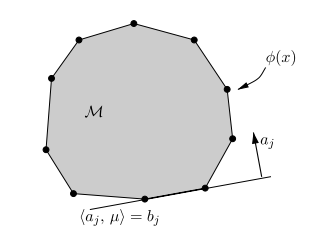
\includegraphics[width=.5\linewidth]{3-5.PNG}
    \caption{
        有限 $|\mathcal{X}^m|$ 下离散随机变量的集合 $\mathcal{M}$ 的图解。
        在这个例子中,集合 $\mathcal{M}$ 是一个与凸包 $\{\phi(x)| ~x \in \mathcal{X}^m\}$ 相关的凸多边形。
        根据 Minkowski-Weyl 定理,这个多边形也能写成有限个半空间的交集,每一个半空间的形式为 $\{\mu \in \mathbb{R}^d| ~\langle a_j, \mu \rangle \geq b_j\}$,$(a_j, b_j) \in \mathbb{R}^d \times \mathbb{R}$。
    }\label{fig:3-5}
\end{figure}

\begin{tcolorbox}
\begin{exam}[伊辛模型的均值参数]

例 3.1 中的伊辛模型的充分统计量为单例函数 $(x_s, s \in V)$ 和 成对函数 $(x_sx_t, (s, t) \in E)$。
充分统计量的向量形式如下:
\begin{equation}
    \phi(x) \coloneqq (x_s, s \in V; x_sx_t, (s, t) \in E) \in \mathbb{R}^{|V| + |E|}
\end{equation}
图 $G$ 的节点和边相应的均值参数对应于特定的边际概率:
\begin{subequations}
\begin{align}
    \mu_s &= \mathbb{E}_p[X_s] = \mathbb{P}[X_s = 1], \quad \forall s \in V \\
    \mu_{st} &= \mathbb{E}_p[X_sX_t] = \mathbb{P}[(X_s, X_t) = (1, 1)], \quad \forall (s, t) \in E
\end{align}
\end{subequations}
可见平均参数向量 $\mu \in \mathbb{R}^{|V|+|E|}$ 由单点上的边际概率($\mu_s$)和边上的成对边际概率($\mu_{st}$)组成。
集合 $\mathcal{M}$ 由 $\{\phi(x), x \in \{0, 1\}^m\}$ 的凸包组成,其中 $\phi(x)$ 由式 (3.30) 给出。
用概率的术语来说,$\mathcal{M}$ 对应于所有定义在 $(X_1, \dots, X_m) \in \{0, 1\}^m$ 上的单点与成对边际概率的集合。
在多面体组合学中,这个集合被称为相关多面体(Correlation Polytope)或者切割多面体(Cut Polytope)。

为了对这些概念有更具体的了解,接下来我们考虑最简单的非平凡情况:即一对连接在一起的变量 $(X_1, X_2)$ 以及它们构成的图。
在这个例子中,集合 $\mathcal{M}$ 是三维空间(两个节点加一条边)中的一个多面体:他是向量 $\{x_1, x_2, x_1x_2| (x_1, x_2) \in \{0, 1\}^2\}$ 的凸包,或者更准确一点
$$conv\{(x_1, x_2, x_1x_2)| (x_1, x_2) \in \{0, 1\}^2\}$$
参见图 \ref{fig:3-6}。

接下来我们考虑一下这个例子的半空间表示 (3.29)。
由初级概率论和一点点计算可以得到三个均值参数 $(\mu_1, \mu_2, \mu_3)$ 必须满足约束 $0 \leq \mu_{12} \leq \mu_i (i = 1, 2)$ 以及 $1+ \mu_{12} - \mu_1 -\mu_2 \geq 0$。
我们可以把这些约束写成矩阵-向量形式
$$\begin{bmatrix}
    0 & 0 & 1 \\
    1 & 0 & -1 \\
    0 & 1 & -1 \\
    -1 & -1 & 1
\end{bmatrix}\begin{bmatrix}
    \mu_1 \\
    \mu_2 \\
    \mu_{12}
\end{bmatrix} \geq \begin{bmatrix}
    0 \\
    0 \\
    0 \\
    -1
\end{bmatrix}$$
这四个约束为图 \ref{fig:3-6} 中的多面体提供了另一种表示形式。

\end{exam}
\end{tcolorbox}

\begin{figure}[htbp]
    \centering
    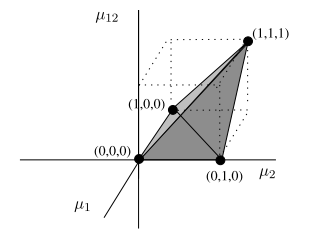
\includegraphics[width=.5\linewidth]{3-6.PNG}
    \caption{
        带有两个变量 $(X_1, X_2) \in \{0, 1\}^2$ 的伊辛模型的集合 $\mathcal{M}$。
        三个均值参数 $\mu_1 = \mathbb{E}[X_1]$,$\mu_2 = \mathbb{E}[X_2]$ 与 $\mu_{st} = \mathbb{E}[X_1X_2]$ 必须满足约束 $0 \leq \mu_{12} \leq \mu_i \quad i = 1, 2$ 以及 $1 + \mu_{12} - \mu_1 - \mu_2 \geq 0$。
        这些约束形成一个四面体,包含在单位超立方体 $[0, 1]^3$ 中。
    }\label{fig:3-6}
\end{figure}

下一个例子涉及纠错编码和二元拟阵理论(Binary Matroid Theory)中出现的一个多面体族:

\begin{tcolorbox}
\begin{exam}[编码字多面体与二元拟阵]

回顾一下例 3.6 中二元线性码的定义:它对应于满足奇偶校验关系
$$\mathbb{C} \coloneqq \{x \in \{0, 1\}^m| \prod_{a \in F}\psi_a(x_{N(a)}) = 1\}$$
的字节串 $x \in \{0, 1\}^m$ 的一个子集,其中每个奇偶校验函数作用在字节串子集 $N(a) \subset \{1, 2, \dots m\}$ 上。
将它视为指数族的时候,充分统计量就是 $\phi(x) = (x_1, x_2, \dots, x_m)$,基础测度为限制在集合 $\mathbb{C}$ 上的计数测度 $\nu$。
因此,这个问题的集合 $M$ 对应于编码字多边形(Codeword Polytope)——即所有编码字的凸包
\begin{align}
    \mathcal{M} &= conv\{x \in \{0, 1\}^m| \prod_{a \in F}\psi_a(x_{N(a)}) = 1\} \nonumber \\
    &= conv\{x \in \mathbb{C}\}
\end{align}

为了进一步做具体的说明,我们接下来考虑由单一奇偶校验关系 $x_1 \oplus x_2 \oplus x_3 = 1$ 定义的 $m = 3$ 位字节串。
图 \ref{fig:3-7}(a) 展示了这个玩具编码的因子图表示。
这个奇偶校验剔除了长度为 $3$ 的 $2^3 = 8$ 种可能字节串的一半取值。
编码字多面体即为 $\{(0, 0, 0), (0, 1, 1), (1, 0, 1), (1, 1, 0)\}$ 构成的凸包,如图 \ref{fig:3-7}(b) 所示,我们有可以使用半空间约束来表示该编码字多面体。
对于这个单奇偶校验码,编码字多面体由四个不等式定义
\begin{subequations}
\begin{align}
    (1-\mu_1) + (1-\mu_2) + (1-\mu_3) &\geq 1 \\
    (1-\mu_1) + \mu_2 + \mu_3 &\geq 1 \\
    \mu_1 + (1-\mu_2) + \mu_3 &\geq 1 \\
    \mu_1 + \mu_2 + (1-\mu_3) &\geq 1
\end{align}
\end{subequations}
这些不等式可以理解为 $(\mu_1, \mu_2, \mu_3)$ 离超立方体 $\{0, 1\}^3$ 的每个被奇偶校验码禁止的顶点的距离至少为 $1$,这点我们将在 8.4.4 小节详细讨论。

对于更长的、附有更多奇偶校验约束的二元线性码,相关的编码字多面体具有更复杂的结构。
编码字多面体在纠错编码问题中起着关键作用,在编码和信息领域对其进行了深入的研究。
任意二元线性码都可以使用二元拟阵来进行识别。
在这种情况下,编码字多面体被称为二元拟阵的循环多面体。
在组合学中,关于这些编码字有着丰富的研究文献。

\end{exam}
\end{tcolorbox}

\begin{figure}[htbp]
    \centering
    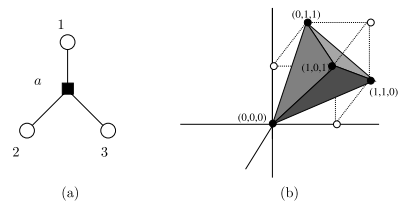
\includegraphics[width=.8\linewidth]{3-7.PNG}
    \caption{
        二元线性码特例 $\mathbb{C} = \{(0, 0, 0), (0, 1, 1), (1, 1, 0), (1, 0, 1)\}$ 相应的集合 $\mathcal{M}$。
        编码由一个简单的奇偶校验码定义。
    }\label{fig:3-7}
\end{figure}

例 3.8 和例 3.9 是某个很一般对象的实例,我们称其为离散图模型的边际多面体。
对于任意节点 $s \in V$ 都具有多元随机变量 $X_s \in \mathcal{X}_s \coloneqq \{0, 1, \dots, r_s-1\}$ 的图模型都可以定义边际多面体。
注意,基数 $|\mathcal{X}_s| = r_s$ 可以随节点而变。
考虑如下以 $\{0, 1\}$ 取值的指示函数所定义的指数族
\begin{align}
    \forall s \in V, j \in \mathcal{X}_s, \quad \mathbb{I}_{s;j}(x_s) &\coloneqq \begin{cases}
        1 & \text{如果} x_s = j \\
        0 & \text{其他}
    \end{cases} \nonumber \\
    \forall (s, t) \in E, (j, k) \quad \mathbb{I}_{st;jk}(x_s, x_t) &\coloneqq \begin{cases}
        1 & \text{如果} (x_s, x_t) = (j, k) \\
        0 & \text{其他}
    \end{cases}
\end{align}
我们将充分统计量 (3.34) 作为标准过完备表示(Standard Overcomplete Representation)。
其过完备性在例 3.2 中讨论过。

上述充分统计量可以使得均值参数具有非常直观的意义:对于每个节点 $s \in V$,都有
\begin{equation}
    \mu_{s;j} = \mathbb{E}_p[\mathbb{I}_j(X_s)] = \mathbb{P}[X_s = j], \quad \forall j \in \mathcal{X}_s
\end{equation}
对于每条边 $(s, t) \in E$
\begin{equation}
    \mu_{st;jk} = \mathbb{E}_p[\mathbb{I}_{st;jk}(X_s, X_t)] = \mathbb{P}[X_s = j, X_t = k], \quad \forall (j, k) \in \mathcal{X}_s \times \mathcal{X}_t
\end{equation}
因此,均值参数对应于节点的单例边际分布 $\mu_s$ 和边的成对边际分布 $\mu_{st}$。
在这种情况下,我们把集合 $\mathcal{M}$ 称为图对应的边际多面体(Marginal Polytope),记为 $\mathbb{M}(G)$。
具体地,它由下式给出
\begin{equation}
    \mathbb{M}(G) \coloneqq \{\mu \in \mathbb{R}^d| ~\exists ~p ~\forall (s; j) \text{满足式 (3.35)}, ~\forall (st; jk) \text{满足式 (3.36)}\}
\end{equation}

例 3.8 中的伊辛模型是边际多面体的一个特例,其节点变量 $X_s \in \{0, 1\}$。
唯一的区别在于边际多面体是在标准过完备指标函数的基础上定义的,而伊辛模型通常都可以参数化为最小指数族的形式。
例 3.9 中的编码字多面体是边际多面体的另一种特殊情况。
在这种情况下,约简需要两个步骤:首先,我们将编码的因子图表示——例如图 \ref{fig:3-7}(a)——转化为一个等价的成对马尔可夫随机场,每个位节点为二元变量,每个因子节点为高阶离散随机变量。
(从因子图转化为两两成对 MRFs 的详细步骤参见附录 E.3。)
和这个成对 MRF 相关的边际多面体只是编码字多面体的提升版。
我们将在后续的章节中更为详细地讨论这些边际多面体的例子。

对于例 3.8 和 3.9 中描述的两个模型,刻画边际多面体所需要的半空间约束的数目 $|\mathcal{J}|$ 非常小(两个例子都是 $|\mathcal{J}| = 4$)。
人们自然会问约束的数目是如何随着图的规模而变化的。
值得说明的是我们随后就能看到所谓的面复杂性(Facet Complexity)其实严重依赖于图结构。
对于树结构来说,任意边际多面体都具有局部约束的特征——只涉及边上的随机变量对——且总数只随图的规模线性增长。
与之形成鲜明对比的是,对于具有环的一般图,其约束是非局部的,并且其数目的增长速率快得惊人。
对于伊辛模型的特殊情况,可以参见 Deza 和 Laurent 的书,里面对相关多面体和切割多面体有详细的描述。
造成统计计算复杂性的一个根本原因在于表示边际多面体的方法是很紧凑的。

\subsection{均值参数在推断问题中的角色}

前面的例子表明均值参数在边际化问题中起着核心作用。
对于多元高斯(例 3.7),计算均值参数化的有效算法为我们提供了高斯均值向量和相关的协方差矩阵。
对于伊辛模型(例 3.8),均值参数完全给定了单点和成对的边际,这也适用于由标准过完备参数化 (3.34) 定义的多元图模型。
更一般地说,从正则参数 $\theta \in \Omega$ 到均值参数 $\mu \in \mathcal{M}$ 的前向映射(Forward Mapping)计算可以看做是指数族模型中推断问题的一个基本类(Fundamental Class)。
尽管对于大多数低维指数族映射的计算很简单,但是对于很多高维指数族来说,这个前向映射的计算极为困难。

反向映射(Backward Mapping),即从均值参数 $\mu \in \mathcal{M}$ 到正则参数 $\theta \in \Omega$ 也有自然的统计解释。
特别地,假设我们有一组样本 $X_1^n \coloneqq \{X^1, \dots, X^n\}$,它们是独立的采样自指数族 $p_{\theta}(x)$,其中 $\theta$ 未知。
如果我们想要估计 $\theta$ 的值,那么根据经典的最大似然原理我们可以通过最大化数据的似然来获得估计值 $\hat{\theta}$,也可以通过取对数等价地最大化量
\begin{equation}
    l(\theta; X_1^n) \coloneqq \frac{1}{n}\sum_{i = 1}^n\log p_{\theta}(X^i) = \langle \theta, \hat{\mu} \rangle - A(\theta)
\end{equation}
其中 $\hat{\mu} \coloneqq \hat{\mathbb{E}}[\phi(X)] = \frac{1}{n}\sum_{i = 1}^n\phi(X^i)$ 为由数据 $X_1^n$ 定义的经验均值参数(Empirical Mean Parameters)向量。
最大似然估计量 $\hat{\theta}$ 是对这个目标函数最大化的解。
需要注意的是,一般而言计算 $\hat{\theta}$ 也是一个难题,因为目标函数中涉及到了对数配分函数 $A$。
下面将会证明,在合适的条件下,最大似然估计量是唯一的,且由统计条件 $\mathbb{E}_{\hat{\theta}}[\phi(X)] = \hat{\mu}$ 确定。
找到这个等式的唯一解等价于计算反向映射 $\mu \mapsto \theta$,从均值参数到正则参数。
一般而言,这个反向映射也需要大量的计算。

\section{对数配分函数 $A$ 的性质}

指数族由四个核心部分组成,充分统计量、正则参数、均值参数以及累积函数(对数配分函数),前三个我们已经有所讨论,现在我们来深入讨论累积函数 $A$ 的一些性质。
$A$ 最重要的性质可能是它的凸性,这是凸分析的领域,其中最重要的是共轭对偶性。
在适当的条件下,函数 $A$ 和它的共轭对偶 $A^*$ ——或者更准确一点地说是他们的导数——在正则参数和均值参数之间建立了一一对应的双射关系。
如前所述,正则参数和均值参数之间的映射关系是高维图模型中各种统计计算的核心挑战。

\subsection{导数和凸性}

回顾一下凸函数的概念,对于一个实值函数 $g$,如果其定义域内任意两个元素 $x, y$ 和任意标量 $\lambda \in (0, 1)$ 满足下列不等式
\begin{equation}
    g(\lambda x + (1-\lambda)y) \leq \lambda g(x) + (1-\lambda)g(y)
\end{equation}
那么 $g$ 是一个凸函数。
从几何的角度来看,这个不等式意味着连接函数值 $g(x)$ 和 $g(y)$ 的线段位于函数图像之上。
如果不等式 (3.39) 对任意 $x \neq y$ 都严格成立,那么这个函数是严格凸(Strictly Convex)的。
(凸函数一些其他的性质参见附录 A.2.5。)
我们先证明对数配分函数在 $\theta$ 上是光滑的、凸的。

\begin{tcolorbox}
\begin{prop}

与任意正则指数族相关的累积函数
\begin{equation}
    A(\theta) \coloneqq \log \int_{\mathcal{X}^m}\exp\langle \theta, \phi(x) \rangle \nu(dx)
\end{equation}
都具有以下性质:

\begin{itemize}
    \item[(a)] 在定义域 $\Omega$ 内具有任意阶导数。
        头两阶导数可以导出随机向量如下累积量(Cumulants):
        \begin{subequations}
        \begin{align}
            \frac{\partial A}{\partial \theta_{\alpha}}(\theta) &= \mathbb{E}_{\theta}[\phi_{\alpha}(X)] \coloneqq \int \phi_{\alpha}(x)p_{\theta}(x)\nu(dx) \\
            \frac{\partial^2 A}{\partial\theta_{\alpha}\partial\theta_{\beta}}(\theta) &= \mathbb{E}_{\theta}[\phi_{\alpha}(X)\phi_{\beta}(X)] - \mathbb{E}_{\theta}[\phi_{\alpha}(x)]\mathbb{E}_{\theta}[\phi_{\beta}(X)]
        \end{align}
        \end{subequations}
    \item[(b)] 此外,$A$ 对 $\theta$ 在其定义域 $\Omega$ 内是凸函数,且在最小表示的情况下是严格凸的。
\end{itemize}

\end{prop}
\end{tcolorbox}

\analysis[证明]
我们假设对 $A$ 的积分定义式 (3.40) 可以进行求导,这个假设可以由支配收敛定理(Dominated Convergence Theorem)得到。
基于这个假设我们有
\begin{align*}
    \frac{\partial A}{\partial \theta_{\alpha}}(\theta) &= \frac{\partial}{\partial \theta_{\alpha}}\{\log\int_{\mathcal{X}^m}\exp\langle\theta, \phi(x)\rangle\nu(dx)\} \\
    &= \frac{[\int_{\mathcal{X}^m}\frac{\partial}{\partial\theta_{\alpha}}\exp\langle\theta, \phi(x)\rangle\nu(dx)]}{[\int_{\mathcal{X}^m}\exp\langle\theta, \phi(x)\rangle\nu(dx)]} \\
    &= \int_{\mathcal{X}^m}\phi_{\alpha}(x)\frac{\exp\langle\theta, \phi(x)\rangle\nu(dx)}{\int_{\mathcal{X}^m}\exp\langle\theta, \phi(u)\rangle\nu(du)} \\
    &= \mathbb{E}_{\theta}[\phi_{\alpha}(X)]
\end{align*}
这就导出了式 (3.41a)。
高阶导数的公式可以用类似的方式进行证明。

观察式 (3.41b) 可知二阶偏导 $\frac{\partial^2A}{\partial\theta_{\alpha}\partial\theta_{\beta}}$ 与协方差元素 $cov\{\phi_{\alpha}(X), \phi_{\beta}(X)\}$ 相等。
因此整个黑塞矩阵(Hessian)$\nabla^2A(\theta)$ 就是随机向量 $\phi(X)$ 的协方差矩阵,其在开集 $\Omega$ 上为半正定的,也就保证了函数的凸性。
如果采用的是最小表示,那么就不存在非零向量 $a \in \mathbb{R}^d$ 和常数 $b \in \mathbb{R}$ 使得 $\langle a, \phi(x)\rangle = b$ 在基础测度 $\nu$ 上几乎处处成立。
这也就表示对于所有的 $a \in \mathbb{R}^d$ 和 $\theta \in \Omega$ 都有 $var_{\theta}[\langle a, \phi(x)\rangle] = a^T\nabla^2A(\theta)a > 0$。
黑塞矩阵在开集 $\Omega$ 上的严格正定意味着函数的严格凸性。
\qed

\subsection{转向均值参数的前向映射}

我们现在来深度探索一下前向映射 $\theta \mapsto \mu$,从正则参数 $\theta \in \Omega$ 定义的分布 $p_{\theta}$ 到与之相关的均值参数向量 $\mu \in \mathbb{R}^d$。
注意到梯度 $\nabla A$ 是一个从 $\Omega$ 到 $\mathbb{R}^d$ 的映射。
命题 3.1 证明了该映射的值域包含在先前定义的可实现的均值参数集合 $\mathcal{M}$ 内
$$\mathcal{M} \coloneqq \{\mu \in \mathbb{R}^d| ~\exists ~p ~s.t. ~\mathbb{E}_p[\phi(X)] = \mu\}$$
以下两个问题对这个映射提出了更深刻的内涵:

\begin{itemize}
    \item[(a)] $\nabla A$ 在什么情况下是一个一一映射?
    \item[(b)] $\Omega$ 在映射 $\nabla A$ 下的像——也就是集合 $\nabla A(\Omega)$ ——在什么情况下覆盖整个集合 $\mathcal{M}$?
\end{itemize}

第一个问题的答案很明了,就是取决于这个指数族是不是最小的。
第二个问题有点微妙:首先需要注意的是,我们在 $\mathcal{M}$ 的定义中均值参数 $\mu \in \mathbb{R}^d$ 可以由任意可能的分布生成,而不仅仅只是充分统计量 $\phi$ 所定义的指数族。
事实证明这个额外的自由度并没有扩大集合 $\mathcal{M}$,正如命题 3.3 所指出的那样,在适当的条件下 $\mathcal{M}$ 中的所有均值参数都可以由指数族分布来实现(边界点可以由这种分布的极限序列来实现)。

我们首先给出第一个问题的答案:

\begin{tcolorbox}
\begin{prop}

当且仅当指数族是最小表示的时候梯度映射 $\nabla A: \Omega \rightarrow \mathcal{M}$ 是一一对应的。

\end{prop}
\end{tcolorbox}

\analysis[证明]
如果表示不是最小的,那么一定存在一个非零向量 $\gamma \in \mathbb{R}^d$ 使得 $\langle \gamma, \phi(x) \rangle$ 在测度 $\gamma$ 上几乎处处为常数。
给定任意一个参数 $\theta^1 \in \Omega$,定义另一个参数向量 $\theta^2 = \theta^1 + t\gamma$,其中 $t \in \mathbb{R}$。
因为 $\Omega$ 为开集,可以选择一个充分小的 $t$ 使得 $\theta^2 \in \Omega$。
在 $\gamma$ 的条件下,密度 $p_{\theta^1}$ 和 $p_{\theta^2}$ 包含相同的概率分布(只是它们的归一化常数不同)。
在这一对上有 $\nabla A(\theta^1) = \nabla A(\theta^2)$,因此 $\nabla A$ 并不是一一对应的。

相反如果表示是最小的,那么根据命题 3.1 $A$ 是严格凸的。
对于任何严格凸可微函数,我们有 $A(\theta^2) > A(\theta^2) + \langle \nabla A(\theta^1), \theta^2-\theta^1 \rangle, \forall \theta^1 \neq \theta^2 \in \Omega$。
调换 $\theta^1$ 和 $\theta^2$ 的位置不等式同样成立。
把这两个不等式加起来可以得到
$$\langle \nabla A(\theta^1) - \nabla A(\theta^2), \theta^1 - \theta^2 \rangle > 0$$
这个不等式对任意不相等的 $\theta^1, \theta^2 \in \Omega$ 都成立,这表明 $\nabla A$ 是一一对应的。
\qed

一般而言,尽管对于过完备表示的梯度映射 $\nabla A$ 并不是一一对应的,但是在 $\nabla A(\Omega)$ 的每个元素和 $\Omega$ 的一个仿射子集之间仍然存在一种一一对应的关系。
具体说来,一个仿射子集就是由映射到同一个均值参数的正则参数组成。
无论是最小表示还是过完备表示,如果 $\mu = \nabla A(\theta)$,那么我们说 $(\theta, \mu)$ 是对偶(Dually Coupled)的。
这个对偶概念在后续的内容里面扮演着重要的角色。

现在我们转向第二个问题,有效正则参数域 $\Omega$ 在梯度映射 $\nabla A$ 下的像 $\nabla A(\Omega)$。
具体说来,这个问题的目标就是确定对于均值向量 $\mu \in \mathcal{M}$ 来说是否存在向量 $\theta = \theta(\mu) \in \Omega$ 满足 $\mathbb{E}_{\theta}[\phi(X)] = \mu$。
这个问题的解其实也很简单:像 $\nabla A(\Omega)$ 只是内点集(Interior) $\mathcal{M}^\circ$。
这个事实值得注意,因为它意味着除了边界点之外的所有均值参数 $\mathcal{M}$ 都可以由指数族的某个成员实现。
为了给这个事实一个直观的解释,给定 $\mathcal{M}$ 中的一个内点均值参数 $\mu$,我们来考虑最大熵问题 (3.3)。
如前所述,如果这个问题的解存在,那么它也必须采用指数族的形式 $p_{\theta}(\mu)$。
此外,从最大熵问题的最优性条件来看,该指数族必须满足矩匹配条件(Moment-matching)$\mathbb{E}_{\theta(\mu)}[\phi(X)] = \mu$。
需要注意的是这些矩匹配条件与定义最大似然问题 (3.38) 的条件是相同的——这一点我们将在下一节中进行讨论,这个事实不是巧合,而是最大熵和最大似然之间的原始-对偶(Primal-Dual)关系的一个结论。

\begin{tcolorbox}
\begin{prop}

在一个最小表示的指数族中,梯度映射 $\nabla A$ 的像是 $\mathcal{M}$ 的内点集,记为 $\mathcal{M}^\circ$。
因此,对于每个 $\mu \in \mathcal{M}^\circ$,都存在某个 $\theta = \theta(\mu) \in \Omega$ 满足 $\mathbb{E}_{\theta}[\phi(X)] = \mu$。

\end{prop}
\end{tcolorbox}

我们在附录 B 中给出了这个结论的证明。
结合命题 3.2,命题 3.3 保证了最小指数族中每个均值参数 $\mu \in \mathcal{M}^\circ$ 都可以由指数族的某个成员密度 $p_{\theta(\mu)}$ 唯一实现。
然而一个典型的指数族 $\{p_{\theta}| \theta \in \Omega\}$ 仅仅描述所有基础测度 $\nu$ 下可能密度的一个严格子集。
在这种情况下,至少也存在一些非指数族的密度 $p$ 能够实现 $\mu$。
指数分布族 $p_{\theta(\mu)}$ 的特点是在所有实现 $\mu$ 的分布集合中具有最大的熵。
$A$ 与最大熵原理的联系可以用共轭对偶函数 $A^*$ 来表示,我们接下来就来讨论它。

\section{共轭对偶:最大似然与最大熵}

共轭对偶(Conjugate Duality)是凸分析的基础,可以通过它自然地导出变分表示。
本节我们讨论对数配分函数 $A$ 和共轭对偶函数 $A^*$ 的关系。
这种共轭关系是由变分原理所决定的,变分原理是本书剩余内容的核心,可以导出各种已知的算法,不论是精确的(例如联合树算法以及它的特例卡尔曼滤波、前后向算法和剥离算法)还是近似的(例如带环图的和积算法、平均场、期望传播、菊池方法、线性规划和半定松弛)。

\subsection{共轭对偶的一般形式}

给定一个函数 $A$,其共轭对偶函数 $A^*$ 定义如下:
\begin{equation}
    A^*(\mu) \coloneqq \sup_{\theta \in \Omega}\{\langle \mu, \theta \rangle - A(\theta)\}
\end{equation}
其中 $\mu \in \mathbb{R}^d$ 为一个固定向量,称为对偶变量,维度和 $\theta$ 相同。
我们选择 $\mu$ 来表示对偶变量是有意为之,因为这些对偶变量就蕴含着均值参数的意义。
事实上,我们已经提到了变分问题 (3.42) 的一种统计解释,右侧就是对数似然 (3.38) 的最优值。
当然,这个最大似然问题只有当向量 $\mu$ 属于 $\mathcal{M}$ 时才有意义,由数据集 $X_1^n = \{X^1, \dots, X^n\}$ 诱导的经验矩矢量 $\hat{\mu} = \frac{1}{n}\sum_{i = 1}^n\phi(X^i)$ 就是一个例子。
我们将优化问题 (3.42) 考虑得更为广泛,包含了任意向量 $\mu \in \mathbb{R}$。
在这种条件下,有必要将 $A^*$ 看作为在拓展实线 $\mathbb{R}^* = \mathbb{R} \cup \{+\infty\}$ 上取值的函数,正如标准的凸分析中一样(参见附录 A.2.5)。

如前所述,共轭对偶函数 (3.42) 与熵密切相关。
回想一下香农熵的定义 (3.2)。
定理 3.4 的主要结果是:当 $\mu \in \mathcal{M}^\circ$ 时,对偶函数 $A^*(\mu)$ 的值恰好是指数分布族 $p_{\theta(\mu)}$ 的负熵,其中 $\theta(\mu)$ 是满足满足关系
\begin{equation}
    \mathbb{E}_{\theta(\mu)}[\phi(X)] = \nabla A(\theta(\mu)) = \mu
\end{equation}
的唯一正则参数向量。
我们也会考虑 $\mu \notin \mathcal{M}^\circ$ 的情况,在这种情况下不可能找到满足关系 (3.43) 的正则参数。
在这种情况下,我们需要对 $A^*(\mu)$ 上界的定义进行更为细致的分析。
事实上,令 $\overline{\mathcal{M}}$ 表示 $\mathcal{M}$ 的闭包,如果 $\mu \notin \overline{\mathcal{M}}$,那么 $A^*(\mu) = +\infty$。
这个事实对于变分方法的使用是至关重要的:它保证任何涉及对偶函数的优化问题可以被简化为一个 $\mathcal{M}$ 上的优化问题。
因此在后续的章节中,我们将大量讨论各种图模型的 $\mathcal{M}$ 结构,如果 $\mathcal{M}$ 的结构过于复杂,我们将会讨论它的近似。

更正式地说,以下在附录 B.2 证明的命题提供了 $A$ 和它的共轭对偶 $A^*$ 之间的关系:

\begin{tcolorbox}
\begin{prop}

\begin{itemize}
    \item[(a)] 对于任意 $\mu \in \mathcal{M}^\circ$,令 $\theta(\mu)$ 表示唯一满足对偶匹配条件 (3.43) 的正则参数
        共轭对偶函数 $A^*$ 具有如下形式
        \begin{equation}
            A^*(\mu) = \begin{cases}
                -H(p_{\theta(\mu)}) & \text{如果} \mu \in \mathcal{M}^\circ \\
                +\infty & \text{如果} \mu \notin \overline{\mathcal{M}}
            \end{cases}
        \end{equation} 
        对于任意边界点 $\mu \in \overline{\mathcal{M}}\setminus\mathcal{M}^\circ$ 我们有 $A^*(\mu) = \lim_{n \to +\infty}A^*(\mu^n)$,其中序列 $\{\mu^n\} \subset \mathcal{M}^\circ$ 收敛到 $\mu$。
    \item[(b)] 在对偶的术语中,对数配分函数也有变分表示
        \begin{equation}
            A(\theta) = \sup_{\mu \in \mathcal{M}}\{\langle\theta, \mu\rangle - A^*(\mu)\}
        \end{equation}
    \item[(c)] 对于所有 $\theta \in \Omega$,式 (3.45) 的上界由满足矩匹配条件
        \begin{equation}
            \mu = \int_{\mathcal{X}^m}\phi(x)p_{\theta}(x)\nu(dx) = \mathbb{E}_{\theta}[\phi(X)]
        \end{equation}
        的唯一向量 $\mu \in \mathcal{M}^\circ$ 取到。
\end{itemize}

\end{prop}    
\end{tcolorbox}

命题 3.4(a) 说明了累积函数 $A$ 和熵之间的对偶性。
接下来对这种关系做如下说明。
第一,有必要认识到 $A^*$ 和通常意义上的熵 (3.2) 有着些许不同:鉴于熵将密度函数映射到实数(因此是一个泛函),对偶函数 $A^*$ 是 $\mathbb{R}^d$ 上的一个拓展实值函数,仅对有效的均值参数 $\mu \in \mathcal{M}$ 有限。

第二,$-A^*(\mu)$ 的值与最大熵问题 (3.3) 的优化值有关,其中 $\mu \in \mathbb{R}^d$ 对约束集进行了参数化。
事件 $A^*(\mu) = +\infty$ 对应于最大熵问题的不可行性。
这是很重要的一点。
约束优化问题是由被优化的集合与被优化的函数定义的。
累积函数的变分表示 (3.45) 采用了最大化问题的形式,我们可以看到满足 $-A^*(\mu) = -\infty$ 的向量 $\mu$ 肯定不是最优解。
因此我们在变分表示 (3.45) 中是对集合 $\mathcal{M}$ 实行最大化而不是 $\mathbb{R}^d$。
这意味着集合 $\mathcal{M}$ 的性质是决定累积函数计算复杂性的关键。

第三,命题 3.4 也阐明了集合 $\Omega$ 和 $\mathcal{M}^\circ$ 之间双射关系的精确性质,这一点适用于所有最小指数族。
特别地,梯度映射 $\nabla A$ 以一一对应的形式将 $\Omega$ 映射到 $\mathcal{M}^\circ$,而对偶函数的梯度 $\nabla A^*$ 则表征了从 $\mathcal{M}^\circ$ 到 $\Omega$ 的逆映射(参见附录 B.3)。
图 \ref{fig:3-8} 展示了基于梯度映射 $(\nabla A, \nabla A^*)$ 的双射关系。

\begin{figure}[htbp]
    \centering
    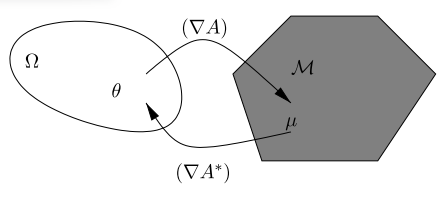
\includegraphics[width=.8\linewidth]{3-8.PNG}
    \caption{
        有效正则参数集合 $\Omega$ 与有效均值参数集合 $\mathcal{M}$ 之间的关系。
        与共轭对偶对 $(A, A^*)$ 相关的梯度映射 $\nabla A$ 和 $\nabla A^*$ 提供了 $\Omega$ 与内点集 $\mathcal{M}^\circ$ 之间的一个双射关系。
    }\label{fig:3-8}
\end{figure}

\subsection{一些简单的例子}

通过一些简单的例子可以很好地理解命题 3.4。
表 \ref{tab:3-2} 提供了几个已知的标量随机变量指数族的共轭对偶 $(A, A^*)$。
对于每个族,该表还列出了 $\Omega \coloneqq dom A$ 以及 $A^*$ 的有效域 $\mathcal{M}$,在这个集合中 $A^*$ 的值是有限的。

\begin{sidewaystable}[htbp]
\caption{
    几个常见的标量指数族的共轭对偶关系
}\label{tab:3-2}
\centering
\begin{tabular}{lcccc}
    \hline
    Family & $\Omega$ & $A(\theta)$ & $\mathcal{M}$ & $A^*(\mu)$ \\
    \hline
    Bernoulli & $\mathbb{R}$ & $\log[1+\exp(\theta)]$ & $[0, 1]$ & $\mu\log\mu + (1-\mu)\log(1-\mu)$ \\
    Gaussian & $\mathbb{R}$ & $\frac{1}{2}\theta^2$ & $\mathbb{R}$ & $\frac{1}{2}\mu^2$ \\
    Gaussian & $\{(\theta_1, \theta_2)| \theta_2 < 0\}$ & $-\frac{\theta_1^2}{4\theta_2^2} - \frac{1}{2}\log{(-2\theta_2)}$ & $\{(\mu_1, \mu_2)| \mu_2 - (\mu_1)^2 > 0\}$ & $-\frac{1}{2}\log[\mu_2 - \mu_1^2]$ \\
    Exponential & $(-\infty, 0)$ & $-\log(-\theta)$ & $(0, +\infty)$ & $-1 - \log\mu$ \\
    Poison & $\mathbb{R}$ & $\exp(\theta)$ & $(0, +\infty)$ & $\mu\log\mu -\mu$ \\
    \hline
\end{tabular}
\end{sidewaystable}

这一小节的剩余部分我们将讨论两个标量的例子。
需要明确的是,从计算的角度来看这两个例子都很平凡——实际上对于大多数标量指数族来说,可以很简单地直接计算正则参数和均值参数之间的映射。
尽管如此,它们还是有助于建立对命题 3.4 的直观理解。
只对主线感兴趣的读者可以直接跳到 3.7 小节,在那里我们将继续对命题 3.4 在推导多元指数族近似推断算法中的作用进行讨论。

\begin{tcolorbox}
\begin{exam}[伯努利模型的共轭对偶性]
    
考虑一个伯努利变量 $X \in \{0, 1\}$:它的分布可以写成指数族的形式,其中 $\phi(x) = x$,$A(\theta) = \log(1+\exp(\theta))$,$\Omega = \mathbb{R}$。
为了验证命题 3.4(a),我们直接计算共轭对偶函数 $A^*$。
通过共轭对偶的定义式 (3.42),对于任意固定的 $\mu \in \mathbb{R}$,我们有
\begin{equation}
    A^*(\mu) = \sup_{\theta \in \mathbb{R}}\{\theta\cdot\mu - \log(1+\exp(\theta))\}
\end{equation}
求导得到驻点条件 $\mu = \exp(\theta)/[1+\exp(\theta)]$,也就是矩匹配条件 (3.43) 在伯努利模型中的特例。
驻点条件在什么情况下有解呢?
如果 $\mu \in (0, 1)$,那么通过一些简单的代数运算我们可以得到唯一解 $\theta(\mu) \coloneqq \log[\mu/(1-\mu)]$。
因为对于伯努利模型来说 $\mathcal{M}^\circ = (0, 1)$,解的存在唯一性就是命题 3.2 和 3.3 的结论。
因为目标函数 (3.47) 是严格凸的,解 $\theta(\mu)$ 就是最优的,将 $\theta(\mu)$ 代入目标式 (3.47) 化简可得
\begin{align*}
    A^*(\mu) &= \mu\log[\frac{\mu}{1-\mu}] - \log[1+\frac{\mu}{1-\mu}] \\
    &= \mu\log\mu + (1-\mu)\log(1-\mu)
\end{align*}
这个就是均值参数为 $\mu$ 的伯努利变量的负熵。
至此我们就验证了在 $\mu \in (0, 1) = \mathcal{M}^\circ$ 情况下的命题 3.4(a)。

现在我们来考虑 $\mu \notin \overline{\mathcal{M}} = [0, 1]$ 的情况,具体地,我们假设 $\mu > 1$。
在这种情况下,优化问题 (3.47) 不存在梯度驻点。
因此上界只能通过取极限 $\theta \to \pm\infty$ 得到。
对于 $\mu > 1$,我们可以得到目标函数在 $\theta \to +\infty$ 时无界。
确实,由 $A$ 的凸性可得 $A(0) = \log 2 \geq A(\theta) + A'(\theta)(-\theta)$。
此外对于所有 $\theta \in \mathbb{R}$ 都有 $A'(\theta) \leq 1$,可得对于 $\theta > 0$ 有 $A(\theta) \leq \theta + \log 2$。
因此对于任意 $\theta > 0$ 我们有
$$\mu\cdot\theta - \log[1+\exp(\theta)] \geq (\mu-1)\theta - \log 2$$
这说明当 $\mu > 1$ 时,目标函数在 $\theta \to +\infty$ 处发散。
同理可得 $\mu < 0$ 的情况,表明 $\mu \notin \overline{\mathcal{M}}$ 时 $A^*(\mu) = +\infty$,证明了命题 3.4(a) 的第二部分。
最后对于边界点 $\mu = 0$ 和 $\mu = 1$,对伯努利模型我们取极限可以得到 $A^*(0) = A^*(1) = 0$。

对于命题 3.4(b) 的验证,由于除非 $\mu \in [0, 1]$, $A^*(\mu) = +\infty$,因此优化问题 (3.45) 简化为
$$\max_{\mu \in [0, 1]}\{\mu\cdot\theta - \mu\log\mu - (1-\mu)\log(1-\mu)\}$$
求解这个凹最大化问题可得其最优值 $\log[1+\exp(\theta)]$,这就证明了命题 3.4(b)。
同理可得最优解 $\mu(\theta) = \exp(\theta)/[1+\exp(\theta)]$ 是唯一的,这就证明了伯努利模型的命题 3.4(c)。

\end{exam}
\end{tcolorbox}

\begin{tcolorbox}
\begin{exam}[指数模型的共轭对偶]
    
考虑指数分布,其指数族形式为 $\phi(x) = x$,$\Omega = (-\infty, 0)$,$A(\theta) = -\log(-\theta)$。
由共轭对偶定义式 (3.42) 可得
\begin{equation}
    A^*(\mu) = \sup_{\theta < 0}\{\mu\cdot\theta + \log(-\theta)\}
\end{equation}
为了得到最优解,我们对 $\theta$ 求导。
我们可以得到驻点条件 $\mu = -1/\theta$,也就是指数分布的矩匹配条件 (3.43)。
因此,对于所有的 $\mu \in \mathcal{M}^\circ = (0, \infty)$,我们有 $A^*(\mu) = -1 - \log(\mu)$。
可以验证 $\mu > 0$ 的指数分布的熵就是 $-A^*(\mu)$。
这就验证了 $\mu \in \mathcal{M}^\circ$ 的命题 3.4。
对于 $\mu \notin \overline{\mathcal{M}}$ ——也就是 $\mu < 0$ ——我们可以验证目标函数 $\mu\theta + \log(-\theta)$ 在 $\theta \to -\infty$ 时无界,从而对于所有 $\mu \notin \mathcal{M}$ 都有 $A^*(\mu) \to +\infty$。
剩下的边界点 $\mu = 0$ 通过定义式 (3.48) 可得 $A*(0) = +\infty$。
还需要注意的是,指数分布 $-1-\log(\mu_n)$ 的负熵对于所有序列 $\mu^n \to 0^+$ 都趋于无穷,这与命题 3.4(a) 一致。
得到对偶 $A^*$ 之后,通过简单的计算就可以得到
$$A(\theta) = -\log(-\theta) = \sup_{\mu > 0}\{\mu\cdot\theta + 1 + \log(\mu)\}$$
最优值在 $\mu = -1/\theta$ 取到。
这就证明了指数分布的命题 3.4(b) 和 (c)。

\end{exam}
\end{tcolorbox}

\section{高维模型的计算困难}

从计算的角度来看,命题 3.4 的基本特性是累积函数的表示 (3.45),以及在均值参数取值 $\mu = \mathbb{E}_{\theta}[\phi(X)]$ 时达到最优的断言 (3.46)。
这表明累积函数 $A$ 和均值参数 $\mu$ 的计算有一个关键的性质:原则上我们可以通过求解变分问题 (3.45) 来计算这两个量。
更令人鼓舞的是,这个优化问题至少从表面上看起来很简单:它是一个凸集上的有限维优化问题,目标函数严格凹且可微。
因此这个优化问题没有局部最优或者其他不好的特性。
这么看来对数配分函数和相关均值参数的计算问题已经解决了,因为我们已经把它“简化”为一个凸优化问题。

在这种情况下,表 \ref{tab:3-2} 中简单的标量例子非常容易误导人,因为它的基本变分问题 (3.45) 有显式解,很容易解决。
相比之下,对于一般的多元指数族,变分表示主要有两个挑战:

\begin{itemize}
    \item[(a)] 在许多情况下,可实现的均值参数约束集合 $\mathcal{M}$ 很难有显式的表征。
    \item[(b)] 负熵函数 $A^*$ 是以一种变分的方式间接定义的,它也同样很难有显式表征。
\end{itemize}

举个例子来说明问题 (a) 提到的 $\mathcal{M}$ 的性质,对于具有离散随机变量 $X \in \{0, 1, \dots, r-1\}^m$ 的马尔可夫随机场,集合 $\mathcal{M}$ 总是一个多面体,也就是我们之前所说的边际多面体。
在这种情况下,集合 $\mathcal{M}$ 至少在原则上可以用有限个线性不等式来刻画。
然而对于一般的图模型来说,这样的不等式随着图模型规模的增长而不断增多。
事实上,除非复杂性理论中的基本猜想被证明是错误的,否则对于一般的离散 MRF 来说在 $\mathcal{M}$ 上优化一个线性函数都是不可能的。
除了约束集合的复杂性之外,问题 (b) 还强调了即使评估单个点 $\mu \in \mathcal{M}$ 的代价函数都是极其困难的,更别说在 $\mathcal{M}$ 上对其进行优化。

为了理解对偶值 $A^*(\mu)$ 的复杂性,注意命题 3.4 只提供了 $A^*$ 一种作为复合映射的隐表征:首先是将 $\mu$ 映射到 $\theta(\mu)$ 的逆映射 $(\nabla A)^{-1}: \mathcal{M}^\circ \to \Omega$,与均值参数为 $\mu$ 的指数族成员相关;其次是从 $\theta(\mu)$ 到相关指数族密度的负熵 $-H(p_{\theta(\mu)})$ 的映射。
$A^*(\mu)$ 值的分解如图 \ref{fig:3-9} 所示。
因此在某个点 $\mu \in \mathcal{M}$ 处计算对偶值 $A^*(\mu)$ 需要计算逆映射 $(\nabla A)^{-1}(\mu)$,这个就已经不简单了,然后再计算熵,这在一般图模型上需要进行高维积分。
这些难点导致需要对 $\mathcal{M}$ 和 $A^*$ 寻求近似。
实际上,如下一章节所示,一大类近似边际化方法都是以对精确变分的近似,然后通过某种消息传递算法来实现的。

\begin{figure}[htbp]
    \centering
    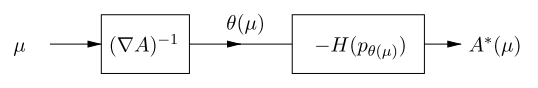
\includegraphics[width=.8\linewidth]{3-9.PNG}
    \caption{
        $A^*$ 作为两个函数复合的分解方块图。
        一个均值参数 $\mu \in \mathcal{M}^\circ$ 首先通过 $(\nabla A)^{-1}(\mu)$ 被映射回正则参数 $\theta(\mu)$。
        再通过相关指数族 $p_{\theta(\mu)}$ 的负熵 $-H(p_{\theta(\mu)})$ 得到 $A^*(\mu)$ 的值。
    }\label{fig:3-9}
\end{figure}

